\documentclass[11pt, oneside]{article}
\usepackage{geometry}
\geometry{letterpaper}
\usepackage{graphicx}
\usepackage{amssymb}
\usepackage{amsmath}
\usepackage{hyperref}
\usepackage{float}
\usepackage{parskip}
\usepackage{fancyref}
\usepackage{fullpage}
\renewcommand{\tabcolsep}{1cm}
\renewcommand{\arraystretch}{1.5}

\title{Hidden Markov Models}
\author{Rapid Learning Session 2014}
\date{}

\begin{document}
\maketitle

This is intended to be a short and informal introduction to HMMs
\footnote{The notation and some parts of this tutorial are based Rabiner LR. (1989) A Tutorial on Hidden Markov Models and Selected Applications in Speech Recognition. \textit{Proceedings of the IEEE}, 77(2):257-286}.

\section{Introduction}
\subsection{What is a hidden Markov model?}
In general, a \textbf{Markov process} is a random process that switches between different states.
%generates values with probabilities that are dependent on the state of the system at that time. 
%The system randomly switches between states 
according to some \textit{transition probabilities}. The probability of being in a particular state at a given time step is dependent only on the the state at the previous time step - this is known as the \textbf{Markov property}. %When we look at data generated from a Markov process, we can see an ordered sequence of states (e.g. A, A, A, B, B) paired with values that were generated at that point in time (e.g. 1, 1, 2, 4, 5). We can use these kinds of data to calculate the transition probabilities between states and also the probabilities of generating particular values given the state of the system at time $t$.

% Maybe we should take this out...probably I think
%A toy example of such a system is the weather throughout the day, depicted in Figure \ref{fig:simple}. 
%\begin{figure}[H]
%\label{fig:simple}
%\centering
%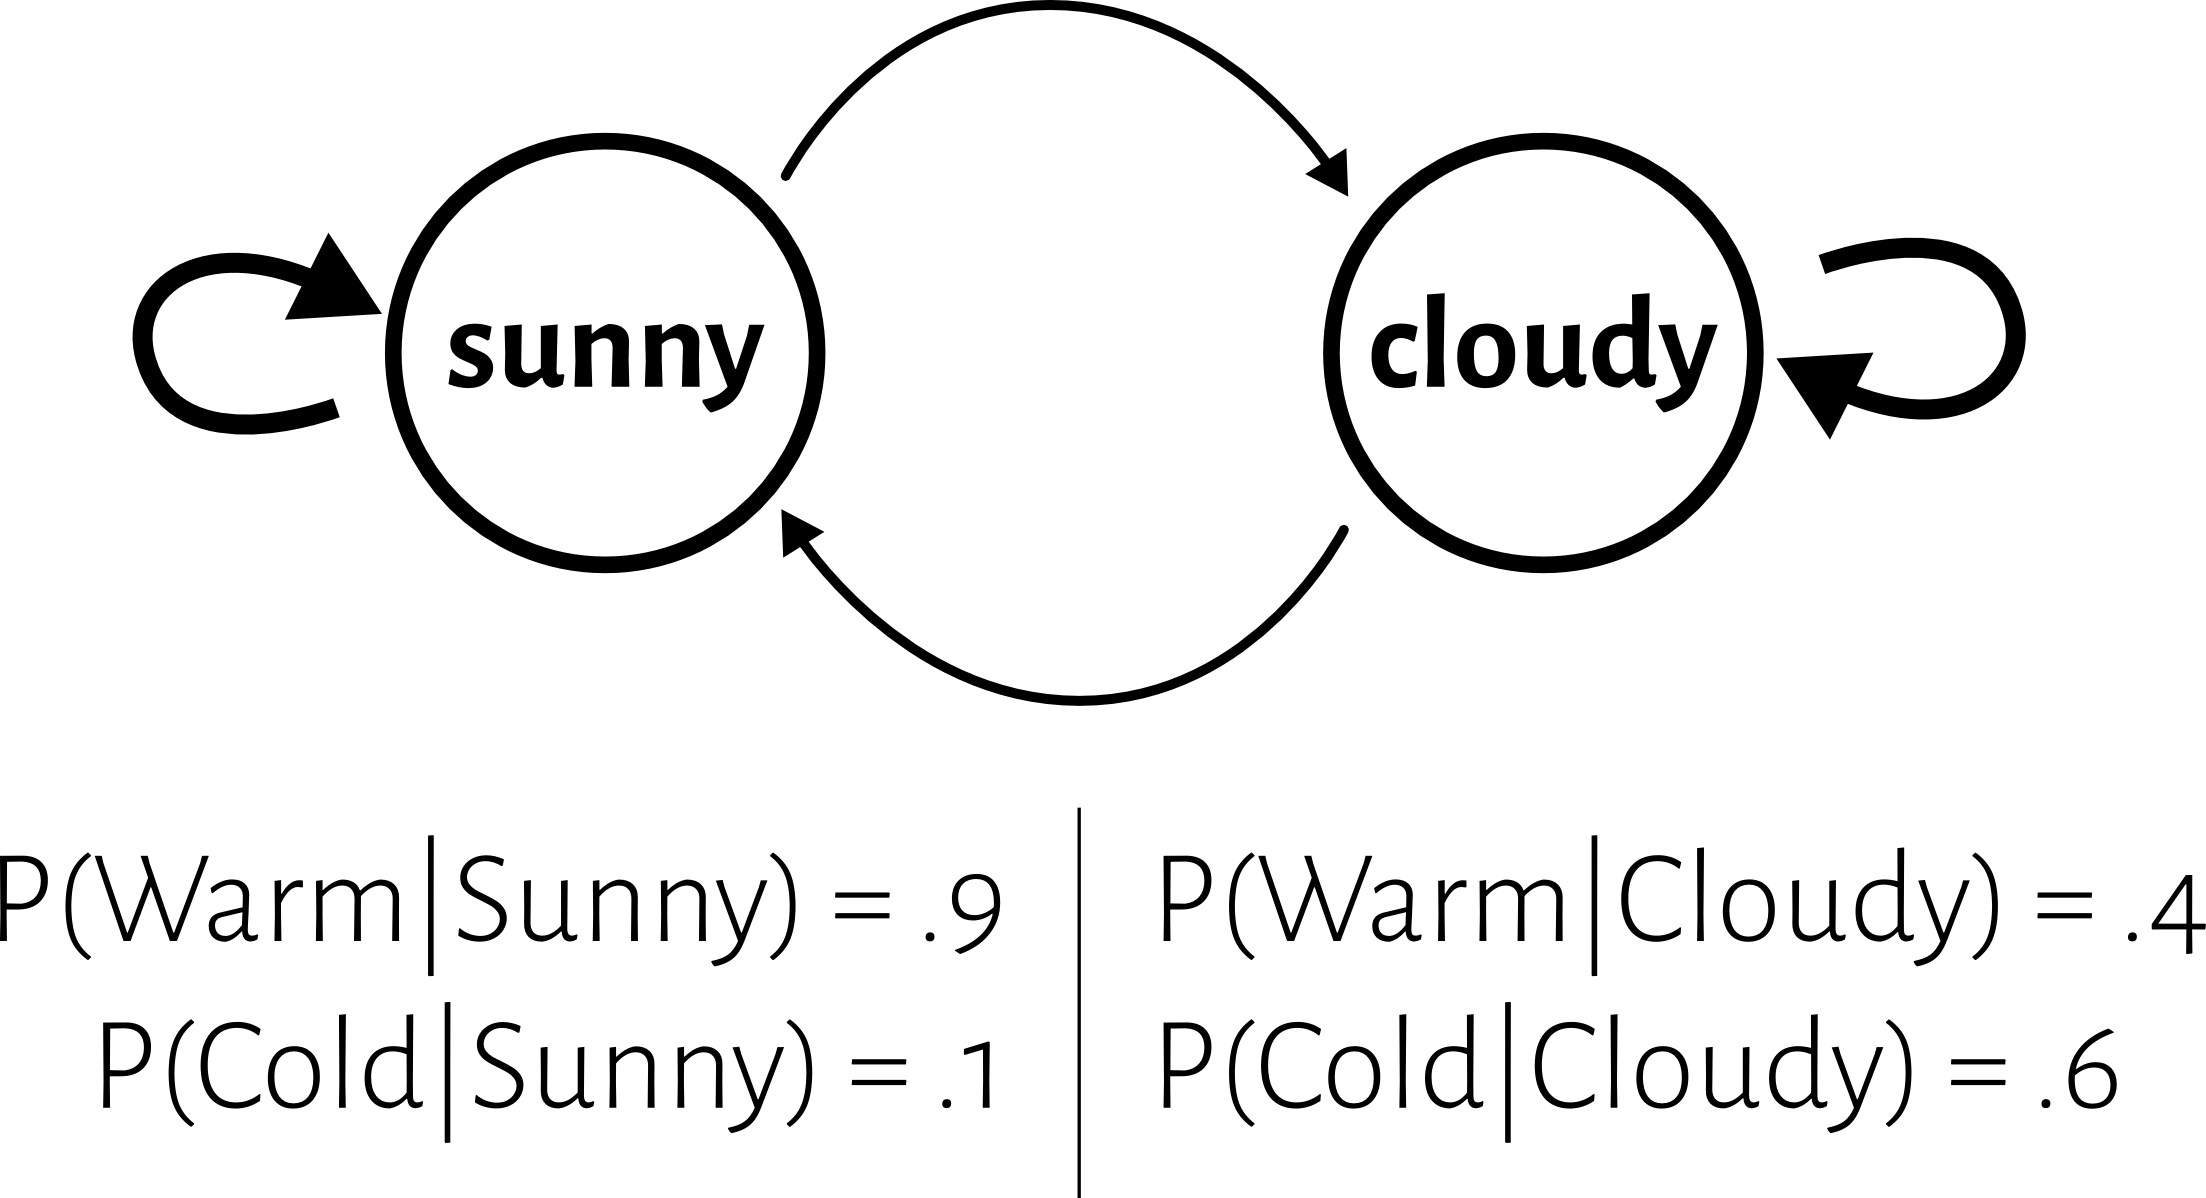
\includegraphics[width=0.5\textwidth]{../figures/g5016.png}
%\caption{A 2-state Markov chain}
%\end{figure}

In contrast, a \textbf{hidden Markov model} is a Markov process with unobserved or ``hidden'' states. However, we do have some noisy information about the states as each state emits observations according to a probability distribution that is characteristic of that state. We see the resulting emissions generated from the process and are not sure of the true underlying state of the Markov process at each given time point. Inferring information about the states of these processes and the probabilities that govern how such processes work has a wide range of applications, particularly for studying sequential data in which we are fairly certain the Markov property is satisfied.

In graphical model notation, an HMM is often represented as in Figure~\ref{fig:pgm}. This clearly shows that the HMM is a series of states with an observation (or emission) generated by each state. Only the emissions are observed and this is depicted by the shading of the respective nodes.

\begin{figure}[H]
\centering
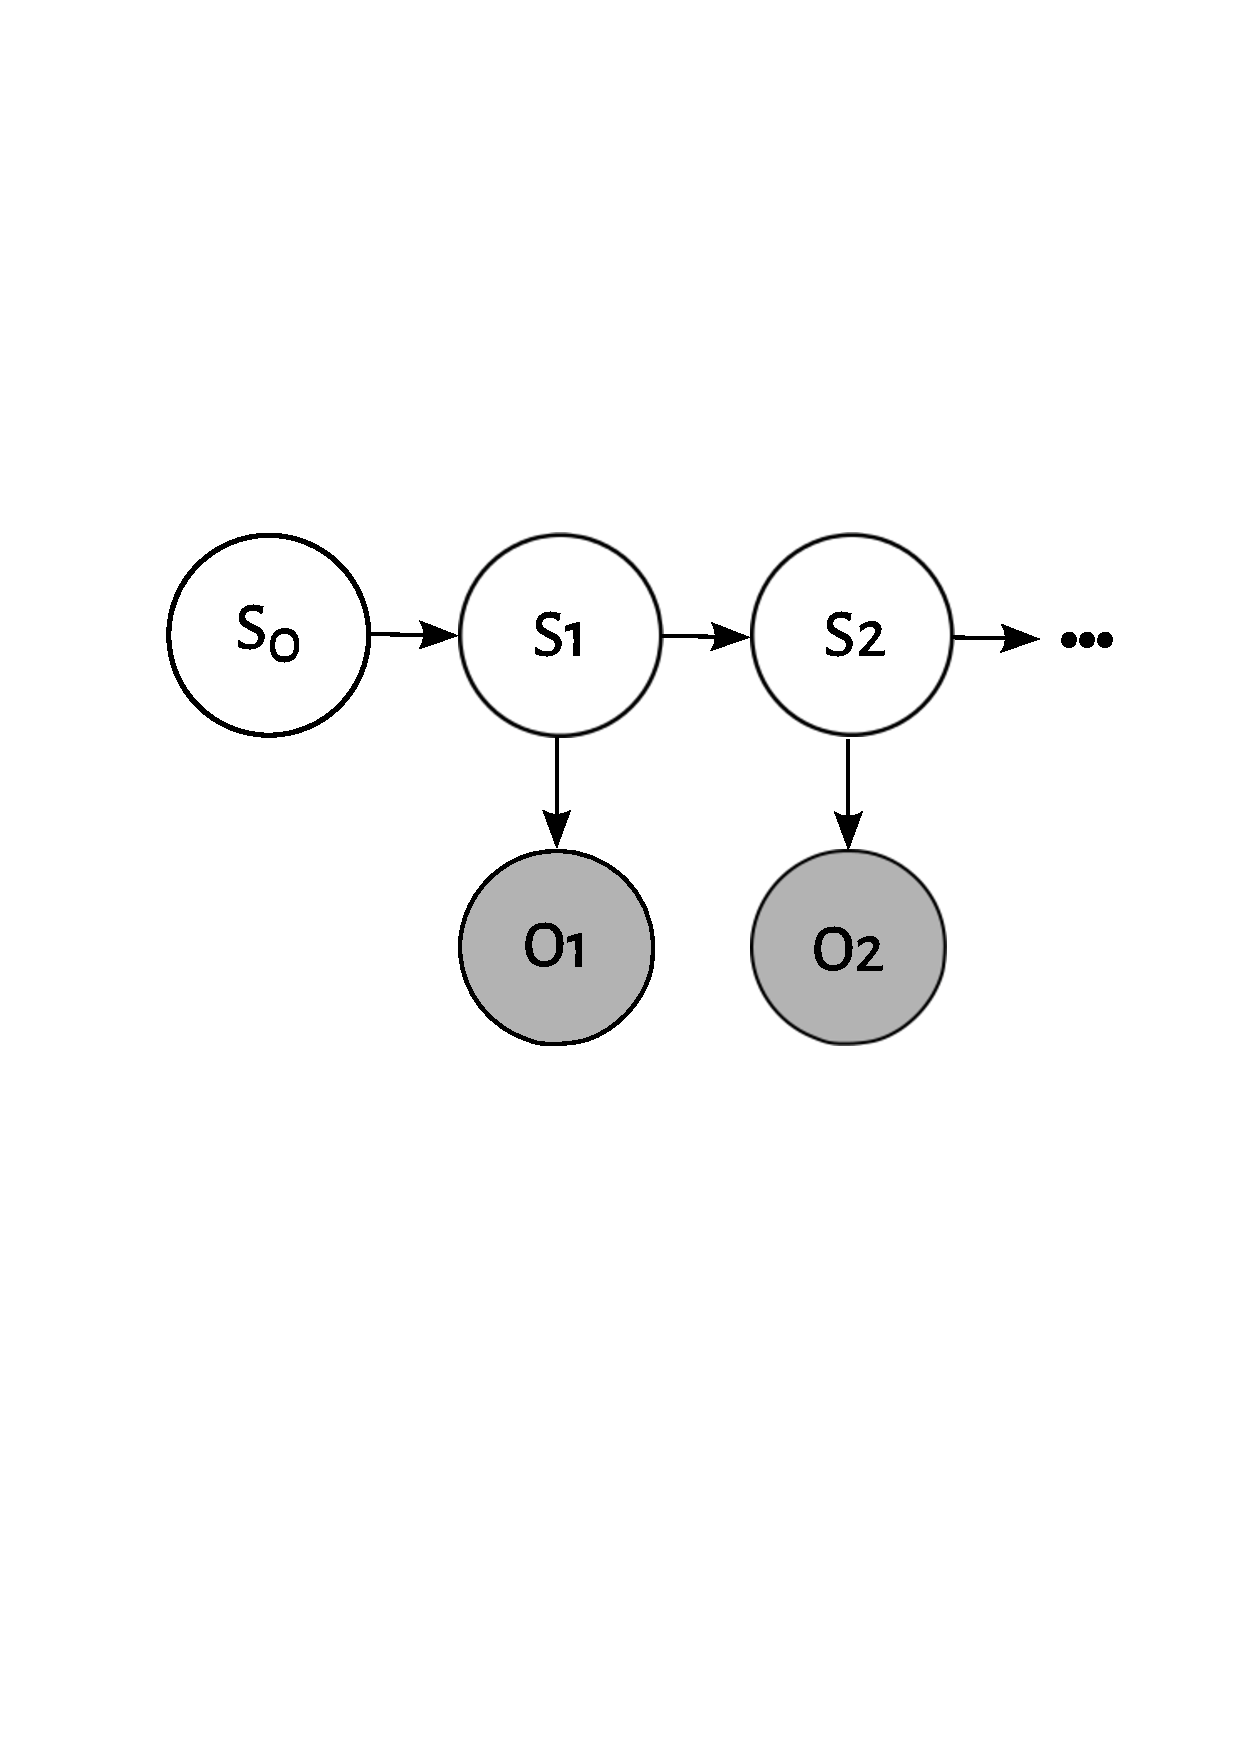
\includegraphics[width=0.45\textwidth]{../figures/hmmTemplate.pdf}
\caption{General graphical model depiction of an HMM}
\label{fig:pgm}
\end{figure}

Sometimes, as in Figure~\ref{fig:gc}, you see an HMM depicted as its underlying Markov Process. Here, the emission probabilities are also shown. In this example we have a two-state HMM that models the GC content of a DNA sequence. 

\begin{figure}[H]
\centering
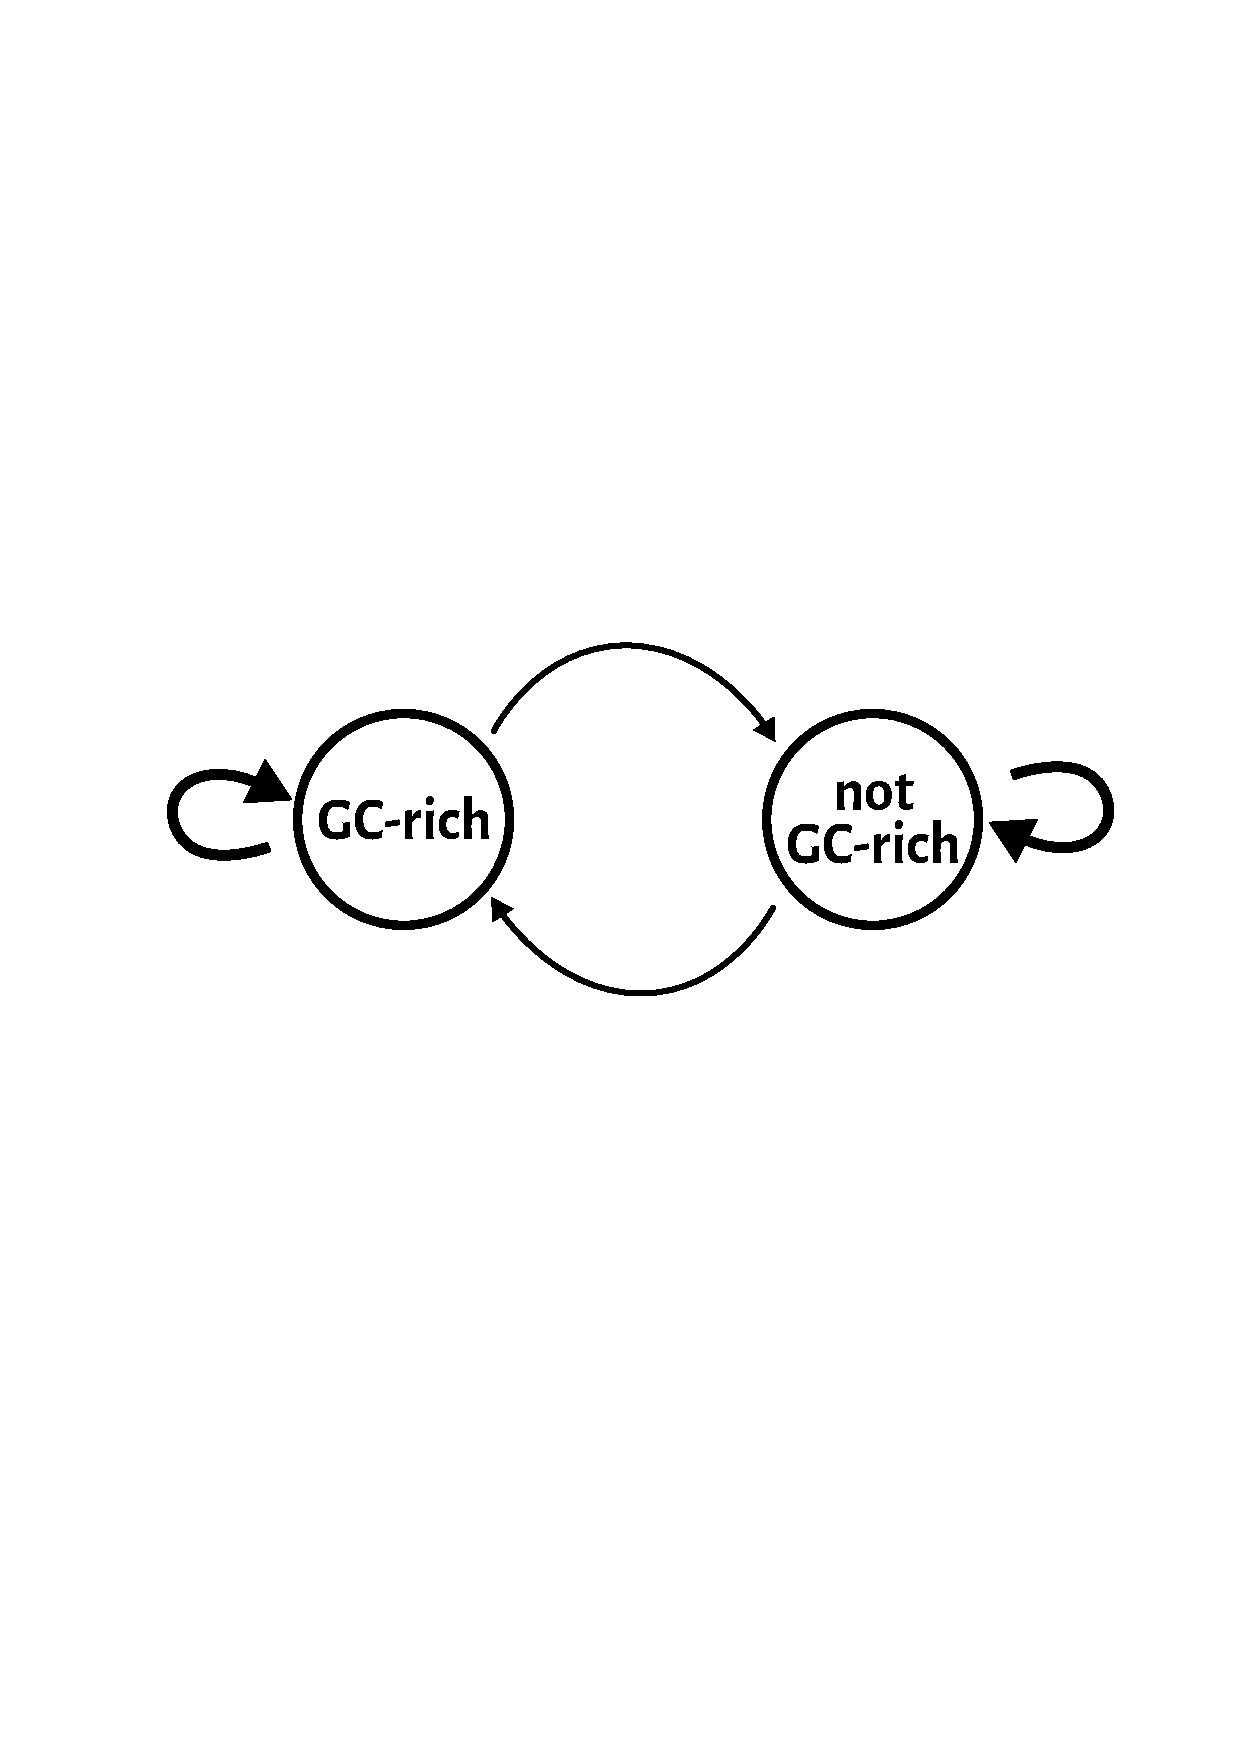
\includegraphics[width=0.55\textwidth]{../figures/hmmGC.pdf}
\caption{Simple GC content HMM.}
\label{fig:gc}
\end{figure}

\subsection{What kind of data is well modeled by a HMM?}
Sequential data are well modeled by HMMs, especially when we are interested labeling sequence segments. Examples of these kinds of data are time series data and DNA sequence data. 

\subsection{Well-known examples of HMMs in biology}

\begin{itemize}
\item Gene finding (GENSCAN: \url{http://genes.mit.edu/GENSCAN.html})
\item Modeling protein sequences and homologs (HMMER: \url{http://hmmer.janelia.org/})
\item Chromatin state annotation (ChromHMM: \url{http://compbio.mit.edu/ChromHMM/})
\end{itemize}

\section{Formal Definition of a HMM}
An HMM is defined by:
\begin{itemize}
\item A set of $s$ states.
\item An alphabet of $n$ possible emissions from each state.
\item A vector of length $s$ where the $i$th entry is the probability of starting in state $i$.
\item An $s\times s$ transition matrix $A$ where $a_{ij}$ is the probability of going from state $i$ to state $j$.
\item An $s \times n$ emission matrix $B$ where $b_{ij}$ is the probability that state $i$ emits symbol $j$.
\end{itemize}

The Markov assumption requires that the state at time $t$ depend only on the state at time $t-1$. We often also assume that the transition and emission probabilities are constant over time.

\section{Algorithms}

There are three main questions we generally want to answer when we have an HMM.

\begin{enumerate}
\item Given the model parameters, what is the probability of a particular observation sequence?
\item Given the model parameters, what is the most likely sequence of states that generated a particular observation sequence?
\item How can we learn the parameters of the model?
\end{enumerate}

The algorithm for each is described in the subsections below. We will use the following notation:

$Q = q_1q_2\cdots q_T$ is a sequence of states of length $T$\\
$O = O_1O_2\cdots O_T$ is an observation sequence of length $T$\\
$a_{q_iq_j}$ is the probability of going from state $q_i$ to state $q_j$\\
$b_{q_i}(O_j)$ is the probability that state $q_i$ emits symbol $O_j$\\
$\pi_{q_i}$ is the probability of starting in state $Q_i$\\
$\lambda$ represents the model parameters, which includes both the emission and transition probabilities

\subsection{The Forward algorithm}

Finding the probability of an observation sequence given the model parameters can be found by summing the probability of seeing that sequence of observations for every possible sequence of states.
\begin{align*}
P(O|\lambda) &= \sum_{\textrm{all possible } Q} P(O,Q|\lambda)\\
&= \sum_{\textrm{all possible } Q} P(O|Q,\lambda)P(Q|\lambda)\\
&= \sum_{q_1q_2\cdots q_T}\pi_{q_1}b_{q_1}(O_1)a_{q_1q_2}b_{q_2}(O_2)\cdots 
a_{q_{T-1}q_T}b_{q_T}(O_T)
\end{align*}

When calculating this quantity, you wouldn't want to actually sum over each of these $N^T$ possible state sequences. Many of the state sequences are similar and you can exploit this to calculate forward probabilities more efficiently. 
\begin{itemize}
\item Define $\alpha_t(i) = P(O_1O_2\cdots O_t, q_t=S_i|\lambda)$.
\item Initialize $\alpha_1(i) = \pi_ib_i(O_1)$.
\item Then $\alpha_{t+1}(j) = \bigl[\sum_{i=1}^N \alpha_t(i)a_ij \bigr]b_j(O_{T+1})$.
\item Finally, $P(O|\lambda) = \sum_{i=1}^N\alpha_T(i)$
\end{itemize}

\subsection{The Viterbi Algorithm}

If we want the single most likely sequence of states we can do something similar to the forward algorithm, but instead of summing over all possible state sequences, we want the max. If you want the sequence of states and not just the max probability, you need to keep track of the states as you go and backtrack at the end to retrieve the sequence. See Rabiner tutorial for details.

%\begin{itemize}
%\item Define $\delta_t(i) = \textrm{max}_{q_1q_2\cdots q_{t-1}} P(q_1q_2\cdots q_t, O_1O_2\cdots O_t|\lambda)$.
%\item Initialize $\delta_1(i) = \pi_ib_i(O_1)$ and $\psi_1(i)=0$.
% need to adjust the part below
%\item Then $\alpha_{t+1}(j) = \bigl[\sum_{i=1}^N \alpha_t(i)a_ij \bigr]b_j(O_{T+1})$.
%\item Finally, $P(O|\lambda) = \sum_{i=1}^N\alpha_T(i)$
%\end{itemize}

\subsection{The Baum-Welch Algorithm}

This is the algorithm used to learn the parameters of an HMM given unlabeled training data. 
It is a special case of the expectation-maximization (EM) algorithm. These types of algorithms work by iterating over two steps: the E-step and the M-step.

In the case of HMMs, if we knew the state that each emission came from, then we could easily infer the emission and transition probabilities (we will do this in Exercise 1). However, in the case of unlabeled data, we do not have this information. The idea is therefore to initialize the parameters with some values then find the most likely state assignment (E-step). With that assignment in hand, we now have labeled data and can use maximum likelihood estimation to update our estimates for the emission and transition parameter values (M-step). We keep iterating between the E- and M-steps until convergence. It is important to note that we may not arrive at an optimal solution. Different initializations of the parameter values can lead to different results.

The inference of the most likely sequence of states (E-Step) is done with the forward-backward algorithm, which returns a probability distribution over the states for each $t$. The backwards probabilities $\beta_t(i)$ are defined like the forwards probabilities $\alpha_t(i)$, but start at the end of the sequence. The probability of being in state $i$ at $t$ is $\frac{\alpha_t(i)\beta_t(i)}{\sum_j \alpha_t(j)\beta_t(j)}$. To use hard EM, you would select the single most likely state (i.e. the state with the highest assigned probability). A better idea is to use soft EM where you keep the soft assignments to states (i.e. the probability distribution).

%\subsection{Caveats}

\section{Exercise 1}
We will use the simple two-state HMM presented in Figure~\ref{fig:gc} for this example.
You have a sequence of observed emissions from this model and you also happen to know which state generated each emission (lucky you!). 
Given these data, you will estimate the parameters of the HMM.

[Use starter code in exercise1.R]

\subsection{Estimate the emission probabilities for each of the two states}
\begin{table}[H]
\centering
\begin{tabular}{|c|c|c|c|c|}
\hline
& A & T & G & C \\\hline
GC rich & & & &  \\\hline
not GC rich & & & & \\\hline
\end{tabular}
\end{table}

\subsection{Estimate the transition probabilities between states}
\begin{table}[H]
\centering
\begin{tabular}{|c|c|c|}
\hline
& GC rich & not GC rich \\\hline
GC rich & &  \\\hline
not GC rich & &  \\\hline
\end{tabular}
\end{table}

How do these parameter estimates compare to the true parameters in Figure~\ref{fig:gc}?

\section{Exercise 2}
Consider an HMM of the same form as before, but this time the model parameters are different. 
Again you observe a sequence of emissions. 
However, this time the states are also unknown. 
This time we will learn the parameters of the HMM without knowing the true sequence of states that generated the observations! 

[Use starter code in exercise2.R]

\textit{Hint}: Think about how you want to initialize the algorithm for the parameter estimation. 

\subsection{Estimate the parameters of the HMM}
Emission probabilities
\begin{table}[H]
\centering
\begin{tabular}{|c|c|c|c|c|}
\hline
& A & T & G & C \\\hline
GC rich & & & &  \\\hline
not GC rich & & & & \\\hline
\end{tabular}
\end{table}

Transition probabilities
\begin{table}[H]
\centering
\begin{tabular}{|c|c|c|}
\hline
& GC rich & not GC rich \\\hline
GC rich & &  \\\hline
not GC rich & &  \\\hline
\end{tabular}
\end{table}

\subsection{Predict the most likely state sequence using the parameters you just estimated}

\end{document} 
